\chapter{Implementation}

	\section{Introduction}

		The objectives of this thesis include not only the development of
		an FBD approach for generalized orthohedral components, but also
		its implementation using an object-oriented programming approach.

		Implementation provides a platform to test, verify and validate the 
		concepts and theory.
		
		This chapter is partitioned into two major units :
			\begin{itemize}
				\item
				{\em Object Oriented Implementation} : This unit deals with the
				use of object-oriented principles as applied to the current 
				research.
				\item
				{\em Graphical User Interface} : This unit deals with the 
				implementation of the user interface using X-Windows Motif 
				toolkit and PHIGS. 

			\end{itemize}

	\section{Object Oriented Implementation}

		The choice of programming paradigm dictates the expressibility and
		the ease with which the concepts can be implemented. The object-oriented
		approach is very well suited for feature-based design implementation,
		due to the natural correspondence between design features and 
		object classes. Object-oriented implementation also provides the
		capability to create application-specific, customized data models
		to extend/alter the current capabilities of the system.

        More specific and complex shapes are derived from the more generalized 
		ones. The data and
        operations specific to a type of block are contained in the
        class that represents that type of block. The functionality specific 
		to the derived shape gets added
        as a specialization. All the classes know how to perform all necessary
		operations on themselves. Another major benefit lies in the 
		re-usability and extendability of the feature library. 
		Dynamic binding allows us to instantiate 
        methods specific to the object type at run time . The virtual function 
		model allows us to develop algorithms for generalized objects 
		which can be overridden at run time by specific
        functions coded for each derived class. These characteristics
        are especially useful in the development of customized feature 
		libraries. 


		\subsection{Object Class Definitions}
		
		C++ is used in this work as a tool to implement the object-oriented 
		feature-based design system. The design of classes and their 
		interaction is too extensive to explain here in full detail
		The top level classes used are shown in Table. ~\ref{cla}.

        \begin{table}[htbp]
        \begin{tabular}{|l|l|}
        \hline
        \bf Class Name  &   \bf Sub-Classes \\
        \hline
        \hline
        {\bf Component} &  Explained later in text \\
        \hline
		Graph	& ComponentGraph, DimensionGraph \\
        \hline
		{\bf Block} & Explained later in text \\
		\hline
		Arc & StrArc, DimArc \\
		\hline
		Face & - \\
		\hline
		Polygon & - \\
		\hline
		Length & - \\
		\hline
		LengthList & - \\
		\hline
		Node & FeatureNode, DimNode, CycleNode, StrongCompNode \\
		\hline
		Plane & - \\
		\hline
		Vertex & - \\
		\hline
		Queue & NodeQueue \\
		\hline
		{\bf Topolink} & Explained later in text \\
		\hline
		Cycle & - \\
		\hline
		StrongComp & - \\
		\hline
		PolygonSet & - \\
		\hline
		Vector & - \\
		\hline
        \end{tabular}
        \caption{Object Classes}
        \label{cla}
        \end{table}

		A description of the most important classes is presented below.

		\subsubsection{ Class Component}

		{\bf Class Component} is the uppermost class in the application. It is 
		conceptually an assembly of blocks along with a set of topological 
		links. In terms 
		of data structure, it is represented as a {\bf Graph} with blocks as
		nodes and topological links as arcs. 
		
		Some of the key functions of this class are discussed here; a full list
		is given in Appendix ~\ref{appclas}.

			\begin{enumerate}
			\item
			{\em Link-Blocks} takes a new block as an argument and appends it
			to the existing list of blocks.
			\item
			{\em Get-max-dimension} traverses the list of blocks and gets
			the maximum dimension of each block; based on this it
			returns the maximum dimension (span) of the component. This function
			is used to set the {\em Display Window} size automatically.
			\item
			{\em Display-by-phigs} displays the model in wireframe.
			\item
			{\em PolygonSet-Display} traverses the block list, collects the
			polygons,forms the polygon-sets and then displays them.
			\item
			{\em Create-default-dim-graphs} traverses all the blocks, collects
			the dimension primitives and forms the default graph
			for the RDG and the SDG.
			\end{enumerate}

		\subsubsection{Class Block}

		{\bf Class Block} is the individual shape unit referred to as
		a ``geometric feature''. It is a rectangular parallelopiped with
		orthohedral geometry. It contains three planes and one length
		along each axis. In terms of data structures, it is represented as
		a {\bf Node}. It contains a pointer to the parent {\bf Component} of 
		which it is a part (Ref. Appendix ~\ref{appblk}).

		Subtractive blocks and blocks whose internal shapes are different
		from their external shape are represented by derived subclasses of
		{\bf Class Block}. The derived classes are shown in
		Fig. ~\ref{shapes} and are discussed below.


	        \begin{figure}[htbp]
%            \centerline{\psfig{figure=shapes.ps,width=5.0in,height=4.0in}}
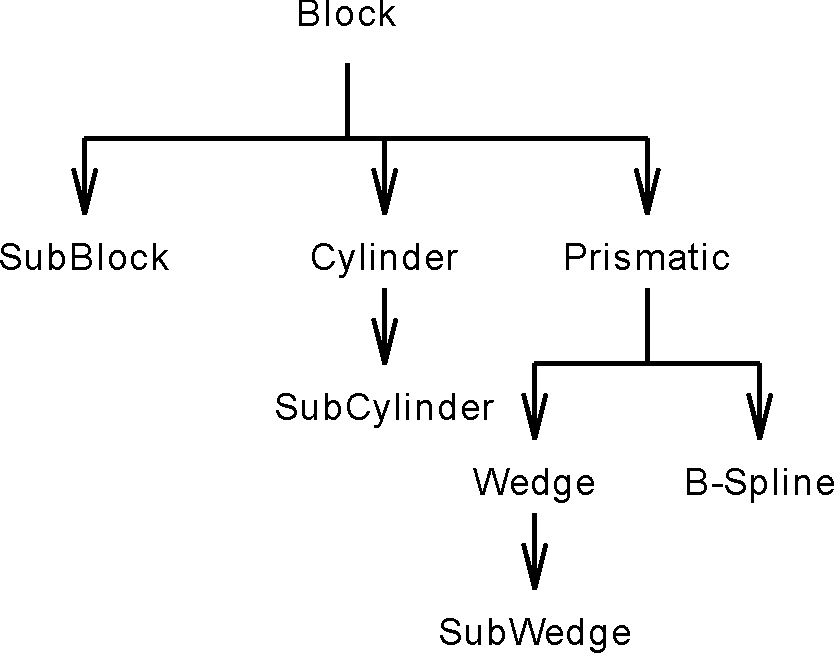
\includegraphics{SHAPES.pdf}
            \caption{Block Hierarchy}
            \label{shapes}
        	\end{figure}

        Some of the key functions of this class are discussed here; a full list
        is given in Appendix ~\ref{appclas}.

            \begin{enumerate}
			\item
            {\em Create-Faces() } which returns six faces of this block.
            \item
            {\em Display-by-phigs()} displays the block in wireframe.
            \item
                {\em Contribute-dim-Faces()}, returns dimensioning planes
                corresponding to the top, bottom and two intersecting middle
                planes.
			\item
			{\em Volume()} returns a positive volume of the block.

            \end{enumerate}


		\begin{itemize}

		\item
        \begin{itemize}
        \item   Class Name :    {\bf Subtractive Block}
        \item   Derived from :  {\bf Block}
        \item   Data Members :	None
		\item	Member functions :

				\begin{itemize}
				\item
				{\em Create-Faces()	} which returns six faces of this block.
				\item
				{\em Display-by-phigs()} which draws the block.
				\item
				{\em Volume()} returns a negative volume of the block.
				\end{itemize}
		\end{itemize}

		\item

        \begin{itemize}
        \item   Class Name :    {\bf Cylinder}
        \item   Derived from :  {\bf Block}
        \item   Data Members :
                \begin{enumerate}
                \item
                axis of the cylinder
                \item
                major-radius
                \item
                minor-radius
                \item
                height along the axis
                \end{enumerate}
		\item	Member functions :
                \begin{itemize}
                \item
                {\em Create-Faces() }, which returns twelve side faces.
                \item
                {\em Volume() }, which returns the volume of the cylinder.
                \item
                {\em Display-by-phigs()}, draws the cylinder.
				\item
				{\em Contribute-dim-Faces()}, returns dimensioning planes
				corresponding to the top, bottom and two intersecting middle
				planes.
                \item
                {\em Create-Polygons() }, which returns two polygons with
                twelve sides each corresponding to the top and the bottom
				faces.
                \end{itemize}
        \end{itemize}


	\item

        \begin{itemize}
        \item   Class Name :    {\bf Subtractive Cylinder}
        \item   Derived from :  {\bf Cylinder}
        \item   Data Members :  None
        \item   Member functions :
                \begin{itemize}
                \item
                {\em Display-by-phigs()} draws the block.
				\item
				{\em Volume()} returns a negative volume of the cylinder.
                \end{itemize}
        \end{itemize}

	\item


        \begin{itemize}
        \item   Class Name :    {\bf Prismatic}
        \item   Derived from :  {\bf Cylinder}
        \item   Data Members :  the axis of extrusion
        \item   Member functions : - (Ref. Appendix ~\ref{appprm}).
        \end{itemize}

	\item

        \begin{itemize}
        \item   Class Name :    {\bf Wedge}
        \item   Derived from :  {\bf Prismatic}
        \item   Data Members :  two butting planes
        \item   Member functions : 

                \begin{itemize}
                \item
                {\em Display-by-phigs()}, which draws the Wedge
				\item
                {\em Create-Polygons()}, which returns a list of five polygons 
				in which three are the side faces and remaining two are top
                and bottom faces.
                \item
                {\em Contribute-dim-Faces()}, which returns the dimensioning 
				planes.
                \end{itemize}
        \end{itemize}

	\item

        \begin{itemize}
        \item   Class Name :    {\bf Subtractive Wedge}
        \item   Derived from :  {\bf Wedge}
        \item   Data Members :  None
        \item   Member functions : - (Ref. Appendix ~\ref{appswed}).
        \end{itemize}

	\item
        \begin{itemize}
        \item   Class Name :    {\bf B-Spline}
        \item   Derived from :  {\bf Prismatic}
        \item   Data Members :  
            \begin{enumerate}
            \item
            Order of the B-spline
            \item
            Knot vector
            \item
            Control Points
            \end{enumerate}
        \item   Member functions :
		(Ref. Appendix ~\ref{appbspline}).
        	\begin{itemize}
                \item
                {\em Display-by-phigs()}, which  draws the block.
        	\end{itemize}
        \end{itemize}

	\end{itemize}

	\subsubsection{Class Topolink}

	{\bf Topolink} : Topolink represents connectivity information between two
	blocks. Figure ~\ref{topo} shows the class hierarchy of the {\bf Class
	Topolink}. It contains following data members :


					\begin{itemize}
					\item	topolink-type :	Type of the topological link
					\item	Block-A-Id	: first block (base block) for
											the topological link
					\item	Block-B-Id	: second block for the topological link
					\end{itemize}

	The operations defined in this class are as follows :
			\begin{itemize}
			\item
        	{\em Get-Block-A-Id()}, which returns block-id of the block-A. 
			\item
        	{\em Get-Block-B-Id()}, which returns block-id of the block-B.
			\item
        	{\em Get-topo-type()}, which returns topolink-type.
			\end{itemize}

            \begin{figure}[htbp]
%            \centerline{\psfig{figure=topo.ps,width=6.0in,height=4.0in}}
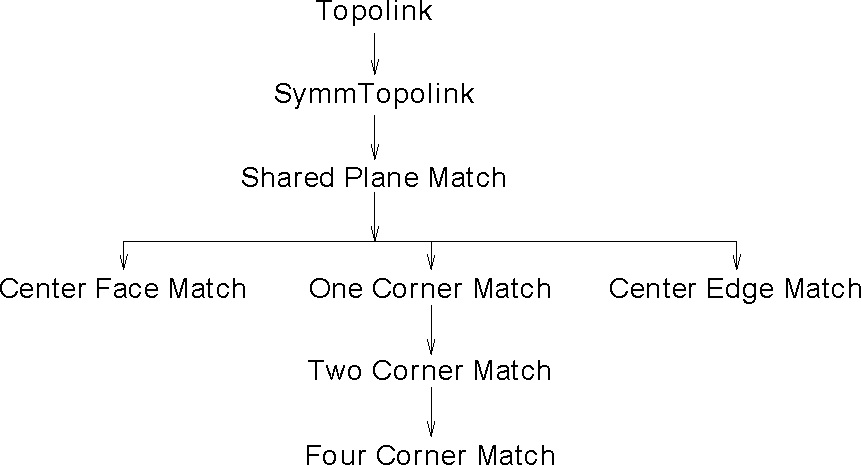
\includegraphics[width=6.0in,height=4.0in]{TOPO.pdf}
            \caption{Topology Hierarchy}
            \label{topo}
            \end{figure}

	The derived classes is shown in Fig. ~\ref{topo} and are discussed below.
	\begin{itemize}

	\item
        \begin{itemize}
        \item   Class Name :	{\bf SymmTopolink}
        \item   Derived from :	{\bf Topolink}
        \item   Data Members :
                    \begin{itemize}
					\item	arcAB :	Arc from node-A to node-B
					\item	arcBA :	Arc from node-B to node-A
                    \end{itemize}
        \end{itemize}

    \item

        \begin{itemize}
        \item   Class Name :	{\bf Shared-Plane-Match}
        \item   Derived from :	{\bf SymmTopolink}
        \item   Data Members :
                    \begin{itemize}
					\item	Plane1-Id :	 Resting plane on parent block-A
                    \end{itemize}
        \end{itemize}


    \item

        \begin{itemize}
        \item   Class Name :	{\bf Center-Face-Match}
        \item   Derived from :	{\bf Shared-Plane-Match}
        \item   Data Members :	None
        \end{itemize}


    \item

        \begin{itemize}
        \item   Class Name :	{\bf Center-Edge-Match}
        \item   Derived from :	{\bf Shared-Plane-Match}
        \item   Data Members :
                    \begin{itemize}
					\item	Plane2-Id :	  Second matched plane on parent block-A
                    \end{itemize}
        \end{itemize}


    \item

        \begin{itemize}
        \item   Class Name :	{\bf One-Corner-Match}
        \item   Derived from :	{\bf Shared-Plane-Match}
        \item   Data Members :
                    \begin{itemize}
					\item	Plane2-Id : second matched plane on parent block-A
					\item	Plane3-Id : third matched plane on parent block-A
                    \end{itemize}
        \end{itemize}

    \item

        \begin{itemize}
        \item   Class Name :    {\bf Two-Corner-Match}
        \item   Derived from :  {\bf One-Corner-Match}
        \item   Data Members :
                    \begin{itemize}
                    \item   Plane4-Id : fourth matched plane on parent block-A
                    \end{itemize}
        \end{itemize}

    \item

        \begin{itemize}
        \item   Class Name :    {\bf Four-Corner-Match}
        \item   Derived from :  {\bf Two-Corner-Match}
        \item   Data Members :
                    \begin{itemize}
                    \item   Plane1-Id : resting plane on parent block-A
                    \end{itemize}
        \end{itemize}


	\end{itemize}


	\subsection{Templates}

	Data structures like linked lists are very commonly used and are well 
	defined in terms of their behavior. They only differ in the {\em type of 
	object} contained in the list. For example, in the current
	implementation, linked lists of blocks, nodes and polygons are used in 
	various algorithms. C++ provides a {\em generic} way of implementing a
	linked list that can contain any type of the object. This is done through
	the use of templates.

	Templates are a relatively new feature of the C++ language. Templates
	provide an effective shorthand notation for defining families of classes
	with similar functions. These families have a similar form but they differ
	in the fact that they are parametrized by data types.

	This work uses the template mechanism to define a family of classes related
	to the {\em List} data structure. It includes {\em Linear Link-list,Queues,}
	and {\em Stacks}. One of the simplest forms of a template class definition
	is given in the following example:%~\cite{blaha} :
		\begin{verbatim}
		template <class T> class class-name
		{
			//	...
		};
		\end{verbatim}
		where T is an element type. Member variables and functions can depend
		on the data type T. T must be explicitly specified when template class
		variables are defined or declared in a program. For example :
		\begin{verbatim}
		template <class T> class Complex
		{
			private :

				T	real;
				T	imaginary;
			public :
				
				Complex( const T & r, const T & i):real(r),imaginary(i){}

				T	Real(){ return real;}
				T 	Img(){	return imaginary;}

		};

		main(){

			Complex <double>	x(1.0,2.0);
			Complex	<int>		j(3,4);

			cout << x.Real()<<" "<<x.Img() <<'\n';
			cout << j.Real()<<" "<<j.Img() <<'\n';

			return 0;
		}
		\end{verbatim}

		Two template class objects are created in the {\em main()} function.
		The object {\em x} is of the data-type {\em Complex $<$ double
		$>$}.
		The object {\em j} is of the data-type {\em Complex$<$int$>$}.
		Template class member functions have the values of their element types
		determined from the element types of the recipient object.

		In the current implementation, template classes such as linked lists,
		stacks and queues are widely used in the implementation of graph
		algorithms such as {\em cycle detection} and {\em strong component
		detection}.

	\section{Graphical User Interface}

	The current implementation uses the Motif toolkit from the Open Software
	Foundation (OSF). The Motif toolkit is based on the X Toolkit Intrinsics 
	(Xt), which is the standard platform on which many of the toolkits
	written for the X Window System are based. Xt provides a library of
	user interface objects called {\it widgets} and {\it gadgets}, which
	provide a convenient interface for creating and manipulating X windows,
	color-maps, events, and other cosmetic attributes of the display. In
	short, widgets can be thought of as building blocks that the programmer
	uses to construct a complete application~\cite{Motif}.

	\subsection{Interface Structure}
		The main window area (see Fig. ~\ref{mainwin}) is made up of four major 
		interface items, viz.:


            \begin{figure}[htbp]
%            \centerline{\psfig{figure=mainwin.ps,width=6.0in,height=4.0in}}
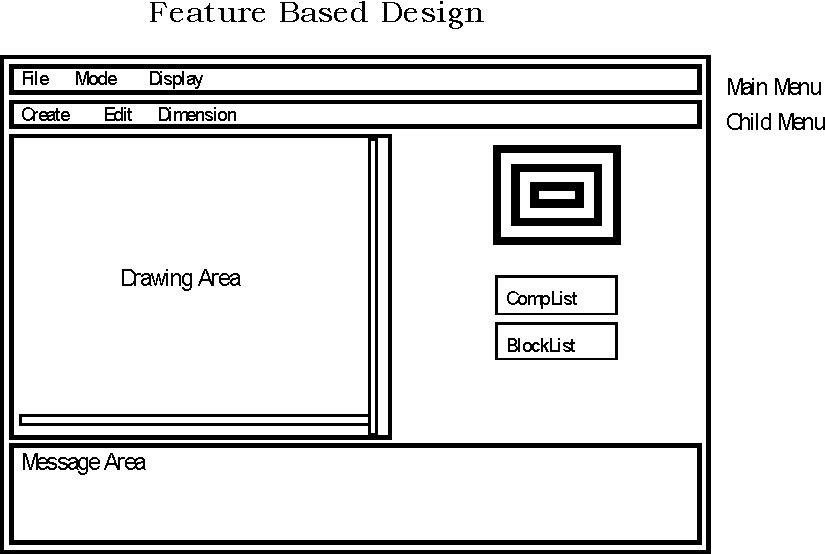
\includegraphics[width=6.0in,height=4.0in]{MAINWIN.pdf}
            \caption{Main Window Interface}
            \label{mainwin}
            \end{figure}

		\begin{itemize}
			\item
			Main Menu : consists of common functionality like file operations,
			display, utility functions, etc.
			\item
			Child Menu : presents either ``design'' options or ``process 
			planning'' options depending on the mode selected.
			\item
			Message Area : displays prompts for input to the user and 
			provides limited on-line help.
			\item
			drawing area : displays the component.
		\end{itemize}

		The {\em Main Menu} has the following options and sub-options :
			\begin{itemize}
			\renewcommand{\thefootnote}{\fnsymbol{footnote}}
			\item
			File : 
				\begin{itemize}
					\item
					New : Begins a new component.
					\item
					Retrieve : Retrieves the component stored in a file
					\item
					Save : Saves the component to a file
					\item
					Exit : Allows the user to exit the system
				\end{itemize}
			\item
			Mode :
					\begin{itemize}
					\item
					Design : Presents design related child menu below this
					main menu.
					\item
					Manufacturing : Presents manufacturing related child menu 
					below this main menu.
					\end{itemize}
			\item
			Display	:
					\begin{itemize}
					\item
					Display-type : Sets display type to polygon-set.
					\item
					Scale 
					\footnotemark[1] \footnotetext[1]{Not supported yet} 
					: Scales the component
					\item
					Rotate \footnotemark[1] : Rotates the component
					\end{itemize}
			\item
			Utilities  \footnotemark[1] : 
					\begin{itemize}
					\item
					Query
					\item
					Mesh
					\item
					Win-Resize
					\item
					Volume
					\item
					Geometric Consistency
					\end{itemize}
			\item
			Settings  \footnotemark[1] : 
					\begin{itemize}
					\item
					Window Settings
					\end{itemize}
			\end{itemize}

		The {\em Child Menu} is of two types viz. ``Design'' and 
		``Manufacturing''.
		The ``Design'' child menu has following options and sub-options
			\begin{itemize}
			\item
			Create : presents the user with following options
				\begin{itemize}
				\item
				New Component : allows the user to create a base block which
				requires purely geometric information
				\item
				Add Block : Presents the shapes in the feature library
				to add to the existing base block. The shapes available are
				\begin{itemize}
				\item
				ADDT-Block : Constructive Block
				\item
				SUBT-Block : Subtractive Block
				\item
				ADDT-Cylinder : Constructive Cylinder
				\item
				SUBT-Cylinder : Subtractive Cylinder
				\item
				ADDT-Wedge : Constructive Wedge
				\item
				SUBT-Wedge : Subtractive Wedge
				\item
				ADDT-B-spline : Constructive B-spline
				\end{itemize}
				\item
				Add Topolink : add a topological link between two pre-existing
				blocks.
				\end{itemize}
			\item
			Edit : 
				\begin{itemize}
				\item
				Geo-Edit : allows the user to edit the geometric data of the 
				component.
				\item
				Add-Geomlink : allows the user to link lengths
				\item
				Delete-Geomlink : allows the user to delink lengths
				\end{itemize}
			\item
			DimTol :
				\begin{itemize}
				\item
				Default-Dim : creates a default dimensioning scheme for the
				current component.
				\item
				Update-Dim : re-creates the dimensioning scheme if the user has
				performed any ``addition'' or ``editing'' changes to the 
				current component.
				\item
				ChgDatum : allows the user to change the datum for dimensioning.
				\item
				Query : allows the user to query the dimension between any two
				planes.
				\end{itemize}
				
			\end{itemize}

    PHIGS is a higher level graphics library that is used to display the 
	components. It provides basic objects and
    associated functionality with the help of which the user can build the 
	model.
    The internal display procedure is abstracted from the user so that
    almost no lower level routines need to be written by the user.

